\newcommand{\balance}{\prg{bal}}
\newcommand{\password}{\prg{pwd}}
\newcommand{\myAccount}{\prg{accnt}}

\section{Lemma 5.7 does hold}

Contrary to what I had said, %If we use the definition of $ \PushAS {y} {A}$ as currently given, then 
 Lemma 5.7 does hold. However, the lemma is nor necessarily applicable to external calls, and thus rule {\sc{ExtCall\_WithSpec\_Weak}} is not necessarily sound -- more in section 2.
 
 
 Here is lemma 5,7 again, with a different number but otherwise identical.

 Lemma \ref{lemma:push:ass:state} states the guarantees given by $\pushSymbolAA$: \  (1) If \ %the current state 
$\sigma$ satisfies  $\PushAS y A$, then   { the callee state (after pushing a frame with the values of $\overline y$) 
will satisfy $A$}. %after pushing a frame with the values of $\overline y$ (here $\PushS {y} {\sigma}$)
(2) is the opposite: {If the callee state (in which we pushed a frame with the values for $\overline y, \overline z$) satisfies $A$, then the
caller state will satisfy 
% (here , conversely,   if a state satisfies  $A$ after a top frame containing the  values of $\overline y$  and some other variables has been pushed % (here \PushSLong {(\overline y, \overline z)} \sigma), 
$\PushAS {y} {A}$. } % will hold {in the caller state}. % after popping that frame.
%, and mapping the free variables of $A$ to their values  in the state  before.

\begin{lemma} 
\label{lemma:push:ass:state}[Lemma 5.7 from main text]
For any state  $\sigma$, assertion $A$, and variables   $\overline y, \overline z$, disjoint with one another:
\\
If  $fv(A)=\emptyset$, then
\begin{enumerate}
 \item
 \label{lemma:push:ass:state:one}
$M, \sigma \models \PushAS {y} {A}\ \ \ \ \ \ \  \ \ \    \Longrightarrow  \ \ \ \ M,  \PushS {y} {\sigma}   \models A$
\item
\label{lemma:push:ass:state:two}
$M, { \PushSLong {(\overline y, \overline z)} {\sigma} } \models\  A \  \ \ \ \Longrightarrow  \ \ \ \ M,  \sigma \models  \PushAS  {y} {A}$
\end{enumerate}
\end{lemma}


The proof of the lemma above hinges on the proof of the following two auxiliary lemmas:

\begin{lemma} 
\label{lemma:lrelavant:push}
For any  states  $\sigma$ and $\sigma'$, addresses $\alpha$, $\overline \alpha$
\begin{itemize}
\item
$\sigma' \in \PushS {\alpha} {\sigma} \ \wedge\ \  \LRelevant \alpha {\sigma'} \ \ \ \Longrightarrow  \ \ \ \exists \alpha_o\in \overline \alpha.\exists f_1,...f_n.[\ {\interpret {\sigma} {\alpha_o.f_1....f_{n}}}=\alpha\ ]\ \ ]$
\end{itemize}
\end{lemma}



\begin{lemma} 
\label{lemma:push:ass:state:P}[5.7 adapted to protection]
For any module  $M$, states  $\sigma$ and $\sigma'$, addresses $\alpha$, $\overline \alpha$, and $\overline {\alpha'}$:
\\
\begin{enumerate}
 \item
 \label{lemma:push:ass:state:one:P}
$\sigma' \in \PushS {\alpha} {\sigma}\ \ \wedge\ \ M,  \sigma \models \protectedFrom {\alpha} {\overline {\alpha}}
\ \ \ \  \ \ \     \Longrightarrow \ \ \ \  \ \ \   M, \sigma' \models \inside  {\alpha} $
\item
\label{lemma:push:ass:state:two:P}
$\sigma' \in \PushSLong{(\overline \alpha, \overline {\alpha'})} {\sigma}\ \ \wedge\ \ M,  \sigma' \models \inside {\alpha} \ \ \ 
\ \ \ \  \ \ \    \Longrightarrow  \ \ \ \  \ \ \   M, \sigma \models \protectedFrom {\alpha} {\overline {\alpha}} $
\end{enumerate}
\end{lemma}

\begin{proof}
The proof hinges on the fact that by definition of $\pushSymbol$, any paths that exist in $\sigma$  also exist in $\sigma'$ -- and vice versa.
Moreover, any objects reachable in ...

In more detail.
%\begin{enumerate}
% \item

\vspace{.2cm}
\noindent
\textbf{Proof of (1)}\\
Assume that\\
(A): \ \ \ $\sigma' \in \PushSLong{ \overline \alpha} {\sigma}$, and \\
(B):\ \ \  $M,  \sigma \models \protectedFrom {\alpha} {\overline \alpha}$ 
 \\
Then, by  (B), and def of relative protection  we have that
\\
(C):\ \ \ $\forall  f_1, ... f_n. \forall \alpha_o \in \overline \alpha.$ \\
$\strut \ \ \ \ \ \ \ \ \  [\ {\interpret {\sigma} {\alpha_o.f_1....f_n}} =\alpha\ 
 \ \ \    \Longrightarrow  \ \ \   M, \sigma \models \internal {\interpret {\sigma} {\alpha_o.f_1....f_{n-1}}}\ \ ]$
\\
By (C), (A), and def $\pushSymbol$ and we have that 
\\
(D):\ \ \ $\forall  f_1, ... f_n. \forall \alpha_o \in \overline \alpha.$ \\
$\strut \ \ \ \ \ \ \ \ \  [\ {\interpret {\sigma'} {\alpha_o.f_1....f_n}} =\alpha\ 
 \ \ \    \Longrightarrow  \ \ \   M, \sigma' \models \internal {\interpret {\sigma'} {\alpha_o.f_1....f_{n-1}}}\ \ ]$
\\
By (D), lemma def. \ref{lemma:lrelavant:push}, and def. of protected, we have 
\\
(E):\ \ \ $M,  \sigma' \models \inside {\alpha}$
\\
Case done!

%\item
\vspace{.2cm}
\noindent
\textbf{Proof of (2)}\\
Assume that\\
(A): \ \ \ $\sigma' \in \PushSLong{(\overline \alpha, \overline {\alpha'})} {\sigma}$, and \\
(B):\ \ \  $M,  \sigma' \models \inside {\alpha}$\\
Then, by  (B), def of protection, and locally reachable  we have that
\\
(C):\ \ \ $\forall  f_1, ... f_n. \forall \alpha_o \in (\overline \alpha, \overline {\alpha'}).$\\
$\strut \ \ \ \ \ \ \ \ \  [\ {\interpret {\sigma'} {\alpha_o.f_1....f_n}} =\alpha\ 
 \ \ \    \Longrightarrow  \ \ \   M, \sigma' \models \internal {\interpret {\sigma'} {\alpha_o.f_1....f_{n-1}}}\ ] ]$
\\
From (C), (B) and by def of $\pushSymbol$ and we have that
\\
(D):\ \ \ $\forall  f_1, ... f_n. \forall \alpha_o \in \overline \alpha.$ \\
$\strut \ \ \ \ \ \ \ \ \  [\ {\interpret {\sigma} {\alpha_o.f_1....f_n}} =\alpha\ 
 \ \ \    \Longrightarrow  \ \ \   M, \sigma \models \internal {\interpret {\sigma} {\alpha_o.f_1....f_{n-1}}}\ \ ]$
\\
By (D) and def. of relative protection, we obtain that\\
(E):\ \ \ $M, \sigma \models \protectedFrom {\alpha} {\overline {\alpha}} $
\\
Case done!
% \end{enumerate}
\end{proof}

\section{Is Lemma 5.7 too weak?}

Lemma 5.7 is used to prove soundness of the rule {\sc{ExtCall\_WithSpec\_Weak}} -- fig. 10 in other document. 
However, Lemma 5.7  is not sufficient:
Lemma 5.7 would not be directly applicable, if arguments that were passed upon the call to a method were not locally reachable at the end of the call.

\subsection{The Difficulty -- an example}

Assume that we have a module with spec $\TwoStatesQ {{x:C}}  {\inside x}{\inside x}$. And assume that in the diagram below,  $2$ has class $C$.

\begin{figure}[htb]
\begin{tabular}{lclclclclcl}
 \hline  \\
\resizebox{3cm}{!}{
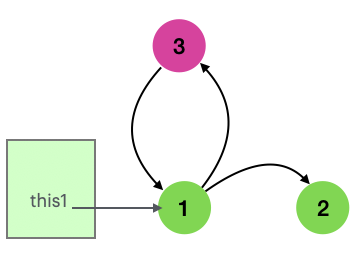
\includegraphics[width=\linewidth]{diagrams/scArgsA.png}
} 
&
\resizebox{3cm}{!}{
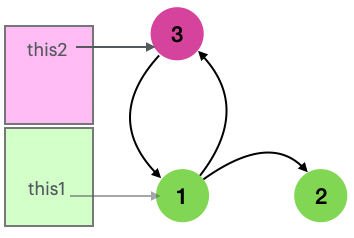
\includegraphics[width=\linewidth]{diagrams/scArgsB.png}
} 
& 
  \resizebox{0.4cm}{!}{
 ...
  } 
&
\resizebox{3cm}{!}{
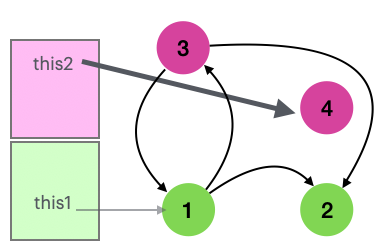
\includegraphics[width=\linewidth]{diagrams/scArgsC.png}
} 
&
\resizebox{3cm}{!}{
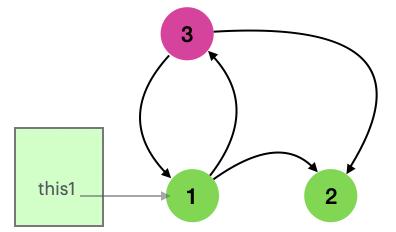
\includegraphics[width=\linewidth]{diagrams/scArgsD.png}
} 
\\
\hline
$..,\sigma_1 \models \protectedFrom {2} {1}$
&
$..,\sigma_2 \models \inside {2}$
&
...
& 
$..,\sigma_{20} \models \inside {2}$
& 
$..,\sigma_{21} \not \models \protectedFrom {2} {1}$
\\  
\hline \hline
\end{tabular}
   \caption{Assignment to parameters -- problem}
   \label{fig:Args}
 \end{figure}

In Fig. \ref{fig:Args} $\sigma_1$ makes a call with argument $3$ (in $\sigma_2$), but by the time that call has finished (in $\sigma_{20}$), $3$ is no longer reachable in $\sigma_{20}$\footnote{I realize  that I changed \prg{this}, but we can esily exted the example, so that we change a different parameter.} . 
Moreover, $2$ is protected from $1$ in $\sigma_1$, while it is not protected from $1$  in $\sigma_{21}$.
But rule   {\sc{ExtCall\_WithSpec\_Weak}} would say that $2$ is protected from $1$ in $\sigma_{21}$.

The above is not a counterexample to lemma \ref{lemma:push:ass:state:P}: We have that $\sigma_{20}\in \PushSLong {4} {\sigma_{21}}$, and thus the lemma  gives that $..,\sigma_{21}   \models \protectedFrom {4} {1}$ -- this is, indeed, true. 
However, rule    {\sc{ExtCall\_WithSpec\_Weak}} would say that $2$ is protected from $1$ in $\sigma_{21}$ --this is {\emph not} true.

The discrepancy arose because the value of the actual parameter, \prg{this}, changed between  $\sigma_2$ and  $\sigma_{20}$

\subsection{1st Solution -- More powerful, and more work}

I believe that a scenario like that in Fig. \ref{fig:Args} cannot happen: Namely, the link from $3$ to $1$ can only be created by an internal call -- remember that ${\encaps {\inside x}}$. Therefore between $\sigma_2$ and $\sigma_{20}$ there must be at least one internal call. But this internal call would ``leak'' $3$, which is forbidden by the spec,

I have started working on such a proof, but it is rather complex, and requires some machinery to keep track of all the frames and the $\inside {\_}$ properties preserved in these frames. 
I am not quite sure how to proceed, though.

\subsection{2nd Solution -- Less powerful, and less work}


An easy way to ensure that   lemma 5.7(2) is applicable to external calls, is if we can ensure  that the arguments that were given at the beginning of a call are still accessible at the end of that call. This is not as restrictive as I had thought originally; we would allow assignments to local variables, but forbid assignments to formal parameters -- Kotlin does this, eg. It would make a operational semantics and the definition of frames a little bit more fiddly though.


\subsubsection{2nd Solution -- Some of the related lemmas and definitions}
We give a formal definition in lemma \ref{lemma:arguments}; we start by defining $\depth{\sigma}$ the depth of a state as the number of frames on $\sigma$'s stack:

\begin{definition}$\strut \ \ \\$

\begin{itemize}
\item
$
\depth{\sigma} \ \triangleq\ n\ \ \  \mbox{iff}\ \ \ \exists h, \phi_1, ... \phi_n.[ \ \sigma = (\phi_1 \cdot ... \phi_n, h) \ ]
$
\end{itemize}
\end{definition}

Our requirement that formal parameters are nor overwritten is 

\begin{lemma}
\label{lemma:arguments}
For any addresses $\overline \alpha$, states $\sigma_1$, ... $\sigma_{n+1}$, and any modules $\Mtwo$ we have
\begin{itemize}
\item
$\forall i\in [1..n]. \Mtwo, \sigma_i \rightarrow \sigma_{i+1}\  \wedge\   \sigma_2\in \PushSLong{ \overline \alpha} {\sigma_1} \ \wedge \ \depth {\sigma_{1}}=\depth{\sigma_{n+1}}\ \ \wedge \ \  \forall i\in [1..n). \depth {\sigma_{i+1}} > \depth {\sigma_{1}}\  $\\
$\strut \ \ \ \ \ \ \ \ \ \ \ \ \  \Longrightarrow\ \  \exists \overline {\alpha'}. \, \sigma_{n}\in \PushSLong { (\overline \alpha,  \overline {\alpha'})} {\sigma_{n+1}}$

\end{itemize}
\end{lemma}

In the lemma above, $\sigma_1$ is a state making a call with arguments $\overline \alpha$, \ \ $\sigma_2$ is the corresponding called state, \ \ $\sigma_3$ ... $\sigma_{n}$ are further states where we do not return from the call in $\sigma_2$, and $\sigma_{n+1}$ is the state right after the call.


\subsubsection{Alternative definitions}

Using the definition of $\depth {\_}$ we can give a (perhaps simpler?) definition of bounded execution:

\begin{definition}[Bounded Execution -- Alternative]
\label{def:shallow:term}
We define relations \    $\leadstoBoundedThree {\Mtwo} {\sigma} {\sigma\bd} {\sigma'}$ \ and\  $\leadstoBounded  {\Mtwo} {\sigma} {\sigma'}$ as:

\begin{itemize}
\item
 $\leadstoBoundedThree {\Mtwo} {\sigma} {\sigma\bd}  {\sigma'}$ \    iff \ \   $\leadstoOrig {\Mtwo} {\sigma} {\sigma'} % $\\
% $\strut  \hspace{3.6cm}\ 
\ \  \wedge \ \    \depth{\sigma}, \depth{\sigma'}\geq  \depth{\sigma\bd}$ 
\item
... as before ...
 \end{itemize}
\end{definition}

Compare this with the original definition

\begin{definition}[Bounded Execution -- Original]
\label{def:shallow:term}
We define relations \    $\leadstoBoundedThree {\Mtwo} {\sigma} {\sigma\bd} {\sigma'}$ \ and\  $\leadstoBounded  {\Mtwo} {\sigma} {\sigma'}$ as:

\begin{itemize}
\item
 $\leadstoBoundedThree {\Mtwo} {\sigma} {\sigma\bd}  {\sigma'}$ \    iff \ \   $\leadstoOrig {\Mtwo} {\sigma} {\sigma'} % $\\
% $\strut  \hspace{3.6cm}\ 
\ \  \wedge $\\
$\strut  \hspace{2.9cm}\ \      \exists \phi,\!\psi,\!\psi_1,\!\psi_2.[ \  \sigma\bd\! =\! (\phi\cdot\psi,\_) \ \wedge \ \sigma\! =\! (\psi_1\cdot \psi, \_)
\ \wedge\ \sigma'\! =\! (\psi_2\cdot \psi, \_)\ \wedge\ {\psi_1,\psi_2\!\neq\! \epsilon}] $ 
\item
....
 \end{itemize}
\end{definition}
%\begin{lemma}
%\label{lemma:arguments:alt}[Alternative expression of Lemma \ref{lemma:arguments}]
%For any addresses $\overline \alpha$, states $\sigma_1$, ... $\sigma_{n+1}$, and any modules $\Mtwo$ we have
%\begin{itemize}
%\item
%$\forall i\in [1..n]. \Mtwo, \sigma_i \leadsto \sigma_{i+1}\  \wedge\   Range(\sigma_2)=\overline \alpha \ \wedge \ \depth {\sigma_{1}}=\depth{\sigma_{n+1}}\ \ \wedge \ \  \forall i\in [1..n). \depth {\sigma_{i+1}} > \depth {\sigma_{1}}\  $\\
%$\strut \ \ \ \ \ \ \ \ \ \ \ \ \  \Longrightarrow\ \  
%\overline \alpha \subseteq Range(\sigma_n)$%\exists \overline {\alpha'}. \, \sigma_{n}\in \PushSLong { (\overline \alpha,  \overline {\alpha'})} {\sigma_{n+1}}$
%
%\end{itemize}
%\end{lemma}



\section{Questions arising from "deeper" modifications of the heap}

 So far, we have considered pretty "flat" examples, where consider  at most one field read. Consider now a module with \prg{Account}s and\prg{Shop}s as below

\begin{lstlisting}[mathescape=true, language=Chainmail, frame=lines]
module $M_{as}$        
  class Password
  
  class Account
    ... as in $\ModA$
    
   class Shop
       field acc: Account
       
       method swap(a:Account)
          this.acc = a
    
\end{lstlisting}
%
  
We use the notation ${\inside{x}}$ to say that $x$ is protected. Assume that we want $M_{as}$   to satisfy

 \begin{tabular}{lcll}
 $S_{as}$   & $\triangleq$   &  $\TwoStatesQ {\prg{s}:\prg{Shop}}  {\inside{\prg{s.acc.pwd}}}  {\inside{\prg{s.acc.pwd}}}$
 \end{tabular}
  
\subsection{Changing footprint}  

Note that the ``footprint'' of $S_{as}$ in the pre-state may be different than that on the post-state. For example, if we have a shop a in the original configuration below,  and execute \prg{s.swap(4)}. then we obtain the configuration to the right. In the original configuration the footprint of \prg{5.acc.pwd} consists of $\{ 1. 2, 3\}$, but in the second configuration it consists of $\{ 1. 4, 5\}$
  
\begin{figure}[htb]
\begin{tabular}{|c|c|}
\hline \\
\resizebox{4.5cm}{!}{
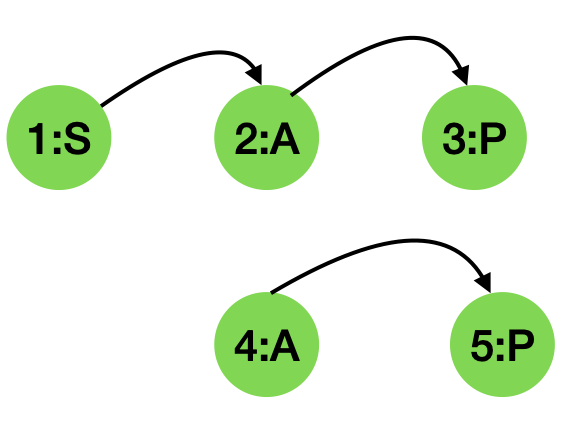
\includegraphics[width=\linewidth]{diagrams/scenarioOne.png}
} 
&
\resizebox{4.5cm}{!}{
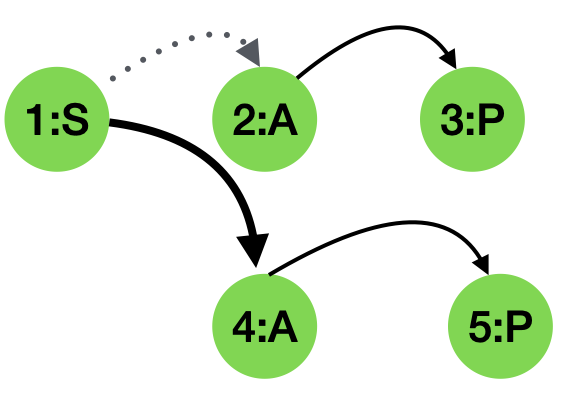
\includegraphics[width=\linewidth]{diagrams/scenarioTwo.png}
} 
\\
\hline
original configuration
&
 configuration after executing \prg{1.swap(4)}
\\
\hline \hline
\end{tabular}
   \caption{changing footprint}
   \label{fig:ScenarioA}
 \end{figure}
 
\subsection{Proving method \prg{swap}}

We can give to  \prg{Swap}  the following pre- and post- condition pair

	$\strut \ \ \ (S_1) \ \ \ \ %\promises
					% {M_{as}}
					 {\mprepostLong 
					 {\inside {this.acc.pwd} \wedge \inside{a.pwd}}
					 {Shop}
					 {swap}
					 {a:Account}
					{\inside {this.acc.pwd}}
					}$
	
Indeed, the method \prg{swap} satisfies $(S_1)$.
Interestingly, it also satisfies the stronger contract:

$\strut \ \ \ (S_2) \ \ \ \ %\promises
					% {M_{as}}
					 {\mprepostLong 
					 {\inside{a.pwd}}
					 {Shop}
					 {swap}
					 {a:Account}
					{\inside {this.acc.pwd}}
					}$



\subsection{A Worry}

Upon first consideration, I worried that external code can call \prg{swap} and expose the password! We show such a scenario in Fig. \ref{fig:ScenarioB}. 
Note that this is happening without changing the identities of the parameters -- as discussed ion section 2!

\begin{figure}[htb]
\begin{tabular}{|c|c|cl}
\hline \\
\resizebox{4.1cm}{!}{
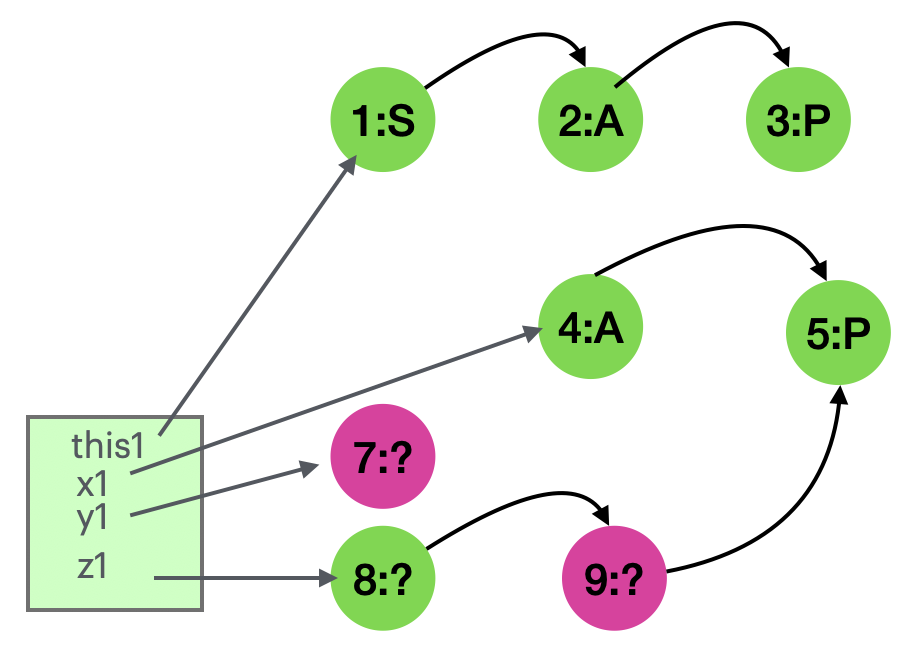
\includegraphics[width=\linewidth]{diagrams/scenarioBOne.png}
} 
&
\resizebox{4.1cm}{!}{
\includegraphics[width=\linewidth]{diagrams/scenarioBTwo.png}
} 
&
\resizebox{4.1cm}{!}{
\includegraphics[width=\linewidth]{diagrams/scenarioBThree.png}
} 
\\
\hline
$\sigma_1$
&
$\sigma_2$
&
$\sigma_3$
\\
\small{$..,\sigma_1 \models {\protectedFrom {\prg{this.acc.pwd}} {\{ \prg{x}, \prg{y}, \prg{z} \}} }$}
&
$..,\sigma_2 \models {\inside {\prg{x.acc.pwd}}}$
&
$..,\sigma_3 \models {\inside {\prg{this.acc.pwd}}} $
\\
\small{$..,\sigma_1 \not\models {\protectedFrom {\prg{x.pwd}} { \prg{z}  }}$} & & 
\\
\hline \hline
\resizebox{4.1cm}{!}{
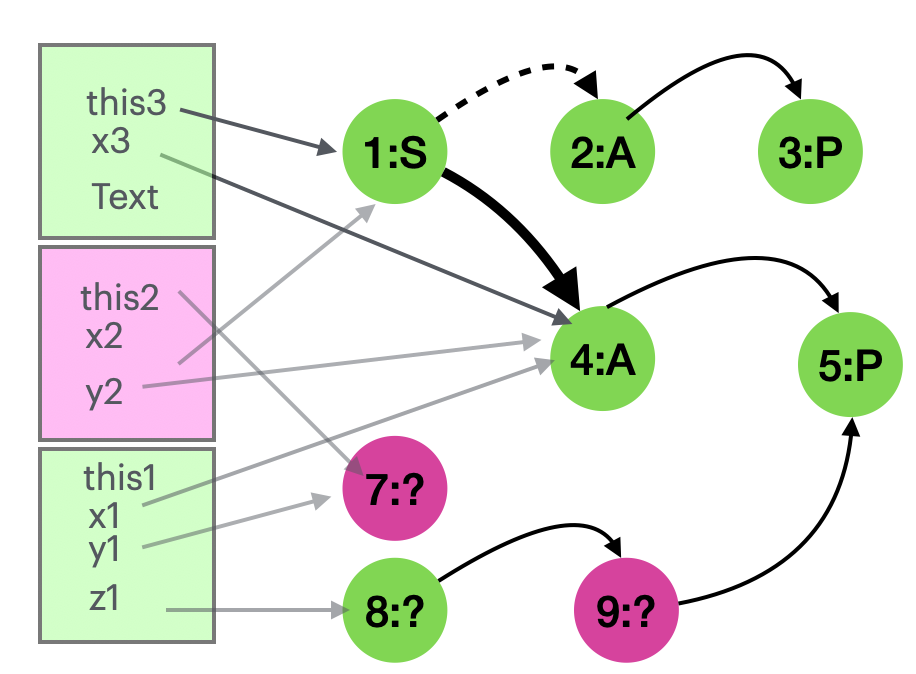
\includegraphics[width=\linewidth]{diagrams/scenarioBFour.png}
} 
&
\resizebox{4.1cm}{!}{
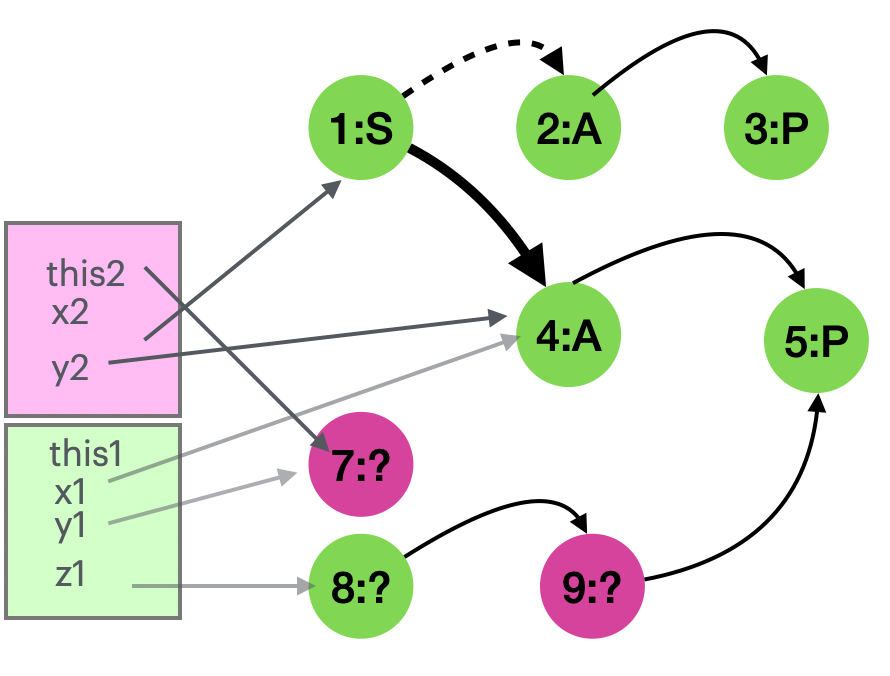
\includegraphics[width=\linewidth]{diagrams/scenarioBFive.png}
}
&
\resizebox{4.1cm}{!}{
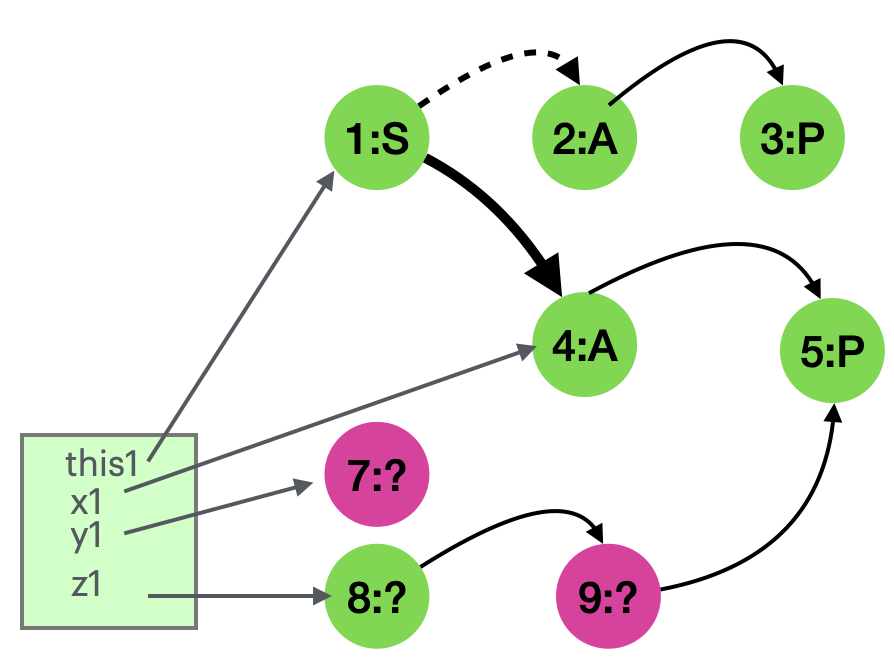
\includegraphics[width=\linewidth]{diagrams/scenarioBSix.png}
} 
\\
\hline 
$\sigma_4$
&
$\sigma_5$
&
$\sigma_6$
\\
$..,\sigma_4 \models {\inside {\prg{this.acc.pwd}}}$
&
$..,\sigma_5 \models {\inside {\prg{x.acc.pwd}}}$
&
\small{$..,\sigma_6 \not\models {\protectedFrom {\prg{this.acc.pwd}} {\{ \prg{x}, \prg{y}, \prg{z} \}} }$}
\\
\hline 
\hline
\end{tabular}
   \caption{calling \prg{swap} and exposing the password?}
   \label{fig:ScenarioB}
 \end{figure}

\subsection{Worry is unfounded?}

The scenario from above is \emph{not} a worry, after all! 
Namely, according to our defintion of well-formed module, the method \prg{swap} need to also satisfy the following, specs:

$\strut \ \ \ (S_3)\ \ \ \ %\promises
					% {M_{as}}
					 {\mprepostLong 
					 {\inside{this.acc.pwd} \ \wedge\ \inside {a.pwd} }
					 {Shop}
					 {swap}
					 {a:Account}
					{\inside {this.acc.pwd}}
					}$
					
					
 And the current method \prg{swap} does not satisfy $(S_3)$!
 
 \subsection{A \prg{swap} that satisfies $(S_3)$ -- more or less!}
 
The only way I can see that \prg{swap}  satisfies $(S_3)$, is if it has been passed already the password of the account. Namely
 
 \begin{lstlisting}[mathescape=true, language=Chainmail, frame=lines]
module $M_{as}$        
  class Password
  
  class Account
    ... as in $\ModA$
    
   class Shop
       field acc: Account
       
       method swap(a:Account,p:Password)
          if (a.pwd == p)
          	{ this.acc = a }    
\end{lstlisting}

And the spec now is:

$\strut \ \ \ (S_4) \ \ \ \ %\promises
					% {M_{as}}
					 {\mprepostLong 
					 {\inside{a.pwd}}
					 {Shop}
					 {swap}
					 {a:Account, p"Password}
					{\inside {this.acc.pwd}}
					}$
 
 But perhaps it is
 
 $\strut \ \ \ (S_5) \ \ \ \ %\promises
					% {M_{as}}
					 {\mprepostLong 
					 {\inside{a.pwd} \wedge \inside{this.acc.pwd}}
					 {Shop}
					 {swap}
					 {a:Account, p"Password}
					 {\inside{a.pwd} \wedge \inside{this.acc.pwd}}
					}$

\subsection{Open Questions}

I have two open questions, but will circulate the document so that we can start the discussion

\begin{enumerate}
\item
I am not sure that  $(S_4)$ or $(S_5)$ are what 
 is what the rule for well-formed modules prescribes or should prescribe!
 \item
 Does this mean that the only way to guarantee a spec of the form 
 
 $\strut \ \ \ (S_6) \ \ \ \ {\mprepostLong 
					 {\inside{x.f}}
					 {...}
					 {m}
					 {...}
					  {\inside{x.f}}
					}$
					
is to pass to \prg{m} the value of \prg{x.f} as an argument?
\end{enumerate}